\documentclass[11pt]{report}
\title{Assignment 3: Task Parallelism in the Genetic Algorithm for the Knapsack problem}
\author{Guilherme Santos      \\
\texttt{fc62533} 
\date{\today}
}
\usepackage[left=1in,right=1in,top=1in,bottom=1in]{geometry}
\usepackage{tikz,pgfplots}
\usepackage{subfig}
\usepackage{caption}
\usepackage{amsmath}
\usepackage{listings}

\lstdefinestyle{mystyle}{
  language=Go, % or the language you are using
  basicstyle=\small\ttfamily,
  numbers=left,
  numberstyle=\tiny,
  frame=single,
  breaklines=true,
  captionpos=b,
}

\begin{document}

\maketitle
\counterwithout{section}{chapter}


The implemented Genetic Algorithm for solving the knapsack problem uses a concurrent architecture based on go-routines and channels in the Go programming language. 
Channels are used to send and receive data between go-routines as well as to synchronize the go-routines to ensure they work correctly.
\\\indent Each individual is calculated in a separate go-routine during the fitness calculation step. The results are delivered to a channel, and the main go-routine receives them. This ensures that the fitness computation occurs concurrently and that the main go-routine obtains the correct results.
Similarly, every operation in the crossover and mutation steps is performed in a separate go-routine. The results are delivered to a channel, where they are received by the main go-routine.
\vspace{15pt}
\begin{lstlisting}[style=mystyle, caption={Fitness calculation step}, label={yourlabel}]
        fitnessResults := make(chan *Individual, POP_SIZE)
        for i := 0; i < POP_SIZE; i++ {
            go func(individual *Individual) {
                individual.MeasureFitness()
                fitnessResults <- individual
            }(population[i])
        }
        for i := 0; i < POP_SIZE; i++ {
            population[i] = <-fitnessResults
        }
        close(fitnessResults)
\end{lstlisting}
\vspace{30pt}

\begin{figure}[h]
  
    \caption*{Execution time with \texttt{N\_GENERATIONS=500} and \texttt{POP\_SIZE=100000}}
   
    \begin{minipage}{0.5\textwidth}
      \centering
      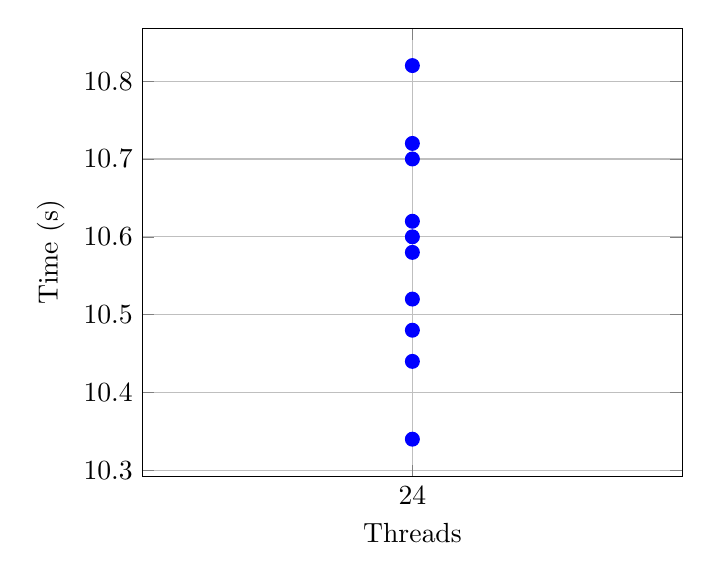
\begin{tikzpicture}
        \begin{axis}[grid=major,xlabel={Threads}, ylabel={Time (s)}, xtick={24}]
          \addplot+[only marks, mark size=2.5pt, mark options={mark=*, blue}]
          coordinates {
            (24,10.70) 
            (24,10.44) 
            (24,10.62) 
            (24,10.72) 
            (24,10.58)
            (24,10.60) 
            (24,10.34) 
            (24,10.52) 
            (24,10.82) 
            (24,10.48)
          };
        \end{axis}
      \end{tikzpicture}
      
      \caption{Threads in Java}
    \end{minipage}%
    \hspace{2em}
    \begin{minipage}{0.5\textwidth}
      \centering
      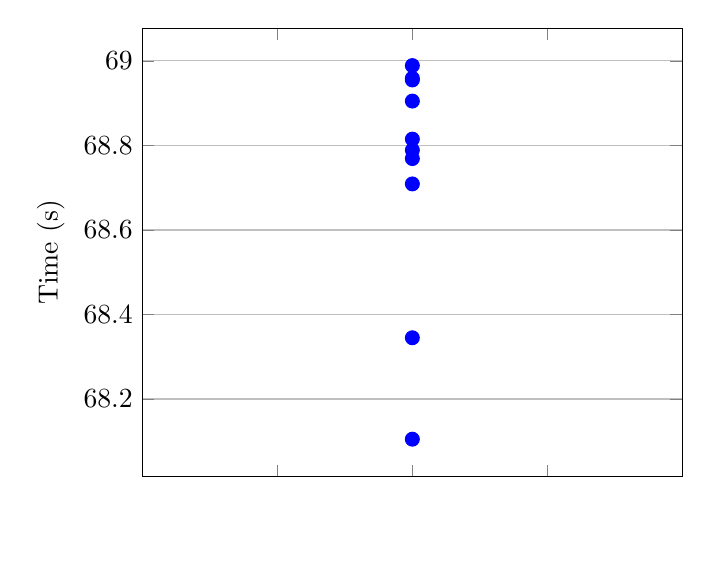
\begin{tikzpicture}
        \begin{axis}[ymajorgrids,xlabel={\phantom{text}}, ylabel={Time (s)},  xticklabels={\phantom{text}}]
          \addplot+[only marks, mark size=2.5pt, mark options={mark=*, blue}]
          coordinates {
            (1,68.955)
            (1,68.959)
            (1,68.989)
            (1,68.789)
            (1,68.105)
            (1,68.769)
            (1,68.815)
            (1,68.709)
            (1,68.345)
            (1,68.905)
          };
        \end{axis}
      \end{tikzpicture}
      \caption{Go-routines and channels}
    \end{minipage}
    \end{figure}

    \begin{tabular}{|c|c|c|c|c|c|}
        \hline
        CPU & Cores & Threads & RAM &  Operating System & Java\\
        \hline
        Intel Core i7-13700 & 16 & 24 & 32GB 6000MHz & Windows 11 & 21\\
        \hline
      \end{tabular}

\end{document}